\documentclass[10pt]{article}

\usepackage{amsthm}
\usepackage{amsfonts}
\usepackage{stmaryrd}
\usepackage{tikz}
\usetikzlibrary{shapes, arrows.meta, positioning}

\tikzstyle{block} = [draw, fill=white, rectangle,
    minimum height=3em, minimum width=2em]
\tikzstyle{sum} = [draw, fill=white, circle, node distance=1cm]
\tikzstyle{input} = [coordinate]
\tikzstyle{output} = [coordinate]
\tikzstyle{pinstyle} = [pin edge={to-,thin,black}]

\newcommand{\Z}{\mathbb{Z}}
\newcommand{\N}{\mathbb{N}}
\newcommand{\B}{\mathbb{B}}
\newcommand{\stream}[1]{\ensuremath{\mathcal{S}_{#1}}}
\newcommand{\zm}{\ensuremath{z^{-1}}}
\newtheorem{theorem}{Theorem}[section]
\newcommand{\code}[1]{\texttt{#1}}
\newcommand{\I}{\mathcal{I}}
\newcommand{\D}{\mathcal{D}}
\newcommand{\distinct}{\mathit{distinct}}

\newcommand{\multiset}[1]{\mathit{multiset}_{#1}}
\newcommand{\set}[1]{\mathit{set}_{#1}}

\title{A model of DDlog}

\begin{document}
\maketitle

\section{Basic notation}

\subsection{Types}

$\N$ is the set of natural numbers, while $\Z$ is the set of integers.

Our language will deal with a set of base types $B$ that includes
$\N$, $\Z$, \code{string}, $\B$ (Booleans), $\mathbf{unit}$.

Derived types include: tuples, vectors (lists), functions.

$$T = B \;|\; T \times T \;|\; T^* \;|\; T \rightarrow T$$

%% We also highlight two special derived types: $\multiset{T}$: finite
%% multisets of elements of type $T$, and $\set{T}$: sets of elements of
%% type $T$.  We call these two particular types \emph{collections}.

A typing context is a map that assigns types to variable names.
$\Gamma = x_1 : T_1, x_2 : T_2, \ldots, x_m : T_m$, where $T_i$ is the
type of variable $x_i$.

\subsection{Multisets}

A monoid $(M, 0_M, +_M)$ is a set $M$ with a distinguished element
$0_M \in M$ and a binary associative operation $+_M : M \times M
\rightarrow M$, such that $a +_M 0 = 0 +_M a = a$ for any $a \in M$.
When clear from the context we drop the index $_M$.  A commutative
monoid has the property that $a + b = b + a$ for all $a, b \in M$.  A
group is a monoid where every element $a \in M$ has a complement $-a
\in M$ such that $a + (-a) = 0$.

Given a monoid (group) $B$, the set of functions between $A$ and $B$
form a monoid (group): M = $A \rightarrow B$, defined by $0_M = (x
\mapsto 0_B)$ and $f +_M g = x \mapsto f(x) +_B g(x)$.  We denote the
\emph{finite} functions between $A$ and $B$ as $B[A]$; these are
functions where $f(x) \not= 0_B$ for at most a finite number of values
of $x \in A$.  Such a function can be denoted by enumerating the
inputs that map to non-zero values: $\{ x_1 \mapsto a_1, \dots, x_n
\mapsto a_n \}$.  The values in $B[A]$ can also be thought as being
key-value maps with keys in $A$ and values in $B$.

In particular, \emph{multisets} with elements of type $A$ are the
functions $\Z[A]$.  Multiset union is just addition in the $\Z[A]$
monoid.  Note that multisets elements can have negative weights.
Multisets form a commutative group, since $\Z$ with addition is a
group.  The zero is the empty multiset $\{\} = \phi$.  Given a
multiset $m \in \Z[A]$ and a value $v \in A$, we overload the array
index notation $m[v]$ to denote the \emph{weight} of the element $v$.

The ``distinct'' function $\distinct: \Z[D] \rightarrow \Z[D]$ projects
a multiset into an underlying set, but \emph{represents the result
  still as a multiset}.  The definition of distinct is given by
$\distinct(m) = \{ x \mapsto 1, m[x] > 0 \} \in \Z[D]$.

\subsection{Streams}

Given a monoid $T$, streams $\stream{T}$ of values of type $T$ are
functions $\N \rightarrow T$.  If $S \in \stream{T}$ is a stream of
values of type $T$, we use the notation $S[t] = S(t) \in T$ is a is
the value of the element of the stream at time $t \in \N$.

The $\zm: \stream{T} \rightarrow \stream{T}$ \emph{delay operator} is
a function from streams to streams, defined as $(\zm(s))[0] = 0_T$,
and $(\zm(S))[t] = S[t - 1]$ for all $t > 0$.

Given a function $f: A \times B \rightarrow C$ one can naturally
extend it to operate on streams $f: \stream{A} \times \stream{B}
\rightarrow \stream{C}$ operating pointwise on time: $f(X, Y)[t] =
f(X[t], Y[t])$ for $t \in \N$.  (This applies to unary functions as
well, which can be extended to operate over a stream pointwise.)

In the rest of this text we only consider streams over multisets: at
each time moment the value of the stream is a multiset.  Since
multisets form a group, addition and subtraction on streams over
multisets of the same type are well-defined.

Given a monoid $M$, integration is an operation from streams to
streams, $\I : \stream{M} \rightarrow \stream{M}$.  The integral of a
stream $S$ is defined using an equation: $\I(S) = \zm(\I(S)) + S$.
Using the notation used for digital filters this equation can be also
written as $\I(S) = S / (1 - \zm)$.  The element of $\I(S)$ at time
$t$ is the (prefix) sum of all elements of $S$ at times up to $t$:
$\I(S)[t] = \sum_{i \leq t} S[t]$, where the sum uses the addition of
the underlying monoid $M$.

Given a group $M$, differentiation is an operation from streams to
streams $\D : \stream{M} \rightarrow \stream{M}$, defined as $\D(S) =
S - \zm(S)$ (we need $M$ to be group in order to have subtraction).
An element of $\D(S)$ (at time $t$) is the difference between the
previous element (time $t-1$) of $S$ and the current (time $t$)
element of $S$.

\begin{theorem}
For a stream $S$ over a commutative group we have $D(I(S)) = S$.
\end{theorem}

\begin{proof}
$\D(\I(S)) = \I(S) - \zm(\I(S)) = (\zm(\I(S)) + S) - \zm(\I(S)) = S$, by
  substituting the definitions of $\D$ and $\I$ and using the
  commutativity of the group.
\end{proof}

\section{DDlog}

\subsection{DDlog types}

\[\frac{\code{A}: T, \code{B}: S}{\code{(A,B)}: T \times S}\]
\[\frac{\code{A}: T, \code{B}: S}{\code{function(x:A):B}: A \rightarrow B}\]
\[\frac{\code{T1}: T_1, \code{T2}: T_2}{\code{T1 | T2} : T_1 \oplus T_2}\]
\[\frac{\code{T1}: T_1, \code{T2}: T_2}{\code{Constructor\{f1: T1, f2:
    T2\}} : \string \rightarrow T_1 \oplus T_2}\]

\subsection{DDlog collections}

DDlog programs consume and produce streams of data.  The outside world
inputs/outputs streams feed to/from DDlog collections.  A DDlog
transaction defines a time step for all the input streams.  On each
transaction commit DDlog updates all output streams.  DDlog programs
only operate on streams.  Some input and output streams are fed
directly to DDlog programs, while others are processed, as described
in this section.

\subsubsection{\code{input stream IS[D]}}

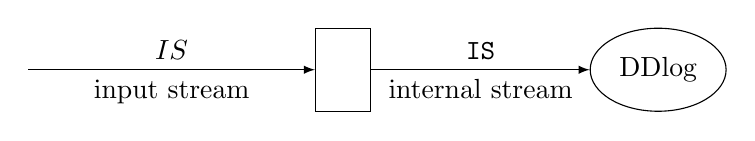
\begin{tikzpicture}[auto, node distance=4cm,>=latex]
    \node [input, name=input] {};
    \node [block, right of=input] (block) {};
    \node [block, shape=ellipse, right of=block] (ddlog) {DDlog};
    \draw [draw,->] (input) -- node {$IS$} (block) node [below,pos=0.5] {input stream};
    \draw [->] (block) -- node {$\code{IS}$}(ddlog) node [below,pos=0.5] {internal stream};
\end{tikzpicture}

A DDlog declaration of \code{input stream IS[D]} declares a (DDlog
internal) stream $\code{IS} \in \stream{\Z[\code{D}]}$, where the
stream's elements are multisets with elements of type \code{D}.  Given
a stream of input values $IS \in \stream{\Z[D]}$, the contents of the
DDlog stream \code{IS} is exactly $IS$.

\subsubsection{\code{output stream OS[D]}}

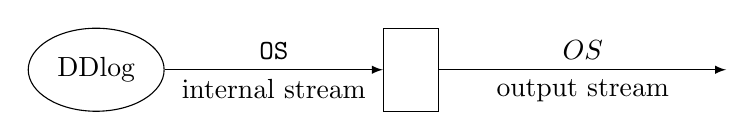
\begin{tikzpicture}[auto, node distance=4cm,>=latex]
    \node [block, shape=ellipse] (ddlog) {DDlog};
    \node [block, right of=ddlog] (block) {};
    \node [output, right of=block] (output) {};
    \draw [draw,->] (ddlog) -- node {\code{OS}} (block) node [below,pos=0.5] {internal stream};
    \draw [->] (block) -- node {$OS$}(output) node [below,pos=0.5] {output stream};
\end{tikzpicture}

As shown in the previous diagram, a DDlog declaration of \code{output
  stream OS[D]} declares an (output) stream $OS \in
\stream{\Z[\code{D}]}$.  The contents of the output stream $OS$ is
exactly the contents of the stream \code{OS}.

\subsubsection{\code{input multiset IM[D]}}

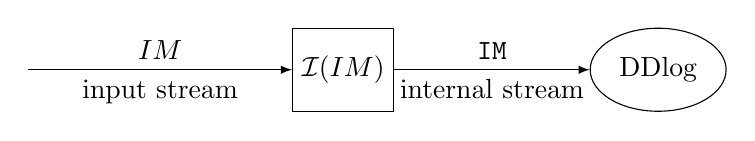
\begin{tikzpicture}[auto, node distance=4cm,>=latex]
    \node [input, name=input] {};
    \node [block, right of=input] (block) {$\I(IM)$};
    \node [block, shape=ellipse, right of=block] (ddlog) {DDlog};
    \draw [draw,->] (input) -- node {$IM$} (block) node [below,pos=0.5] {input stream};
    \draw [->] (block) -- node {$\code{IM}$}(ddlog) node [below,pos=0.5] {internal stream};
\end{tikzpicture}

A DDlog declaration of \code{input multiset IM[D]} declares a stream
$\code{IM} \in \stream{\Z[\code{D}]}$.  Given a stream of input values
$IM \in \stream{\Z[\code{D}]}$, the contents of \code{IM} is given by
$\code{IM} = \I(MI)$, the integral of the stream of inputs.

\subsubsection{\code{output multiset OM[D]}}

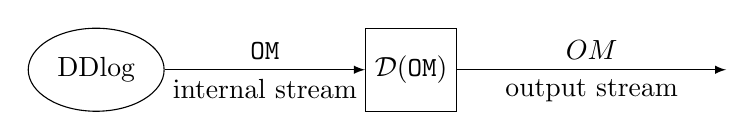
\begin{tikzpicture}[auto, node distance=4cm,>=latex]
    \node [block, shape=ellipse] (ddlog) {DDlog};
    \node [block, right of=ddlog] (block) {$\D(\code{OM})$};
    \node [output, right of=block] (output) {};
    \draw [draw,->] (ddlog) -- node {\code{OM}} (block) node [below,pos=0.5] {internal stream};
    \draw [->] (block) -- node {$OM$}(output) node [below,pos=0.5] {output stream};
\end{tikzpicture}

A DDlog declaration of \code{output multiset OM[D]} declares a stream
$OM \in \stream{\Z[\code{D}]}$.  The contents of the (output) stream
$OM$ is given by $OM = \D(\code{OM})$, the derivative of the stream
\code{OM}.

\subsubsection{\code{input relation IR[D]}}

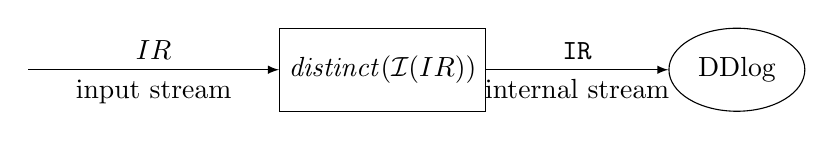
\begin{tikzpicture}[auto, node distance=4.5cm,>=latex]
    \node [input, name=input] {};
    \node [block, right of=input] (block) {$\distinct(\I(IR))$};
    \node [block, shape=ellipse, right of=block] (ddlog) {DDlog};
    \draw [draw,->] (input) -- node {$IR$} (block) node [below,pos=0.5] {input stream};
    \draw [->] (block) -- node {$\code{IR}$}(ddlog) node [below,pos=0.5] {internal stream};
\end{tikzpicture}

A DDlog declaration of \code{input relation IR[D]} declares a stream
$\code{IR} \in \stream{\Z[\code{D}]}$.  The elements of the stream
\code{IR} are defined by $\code{IR} = \distinct(\I(IR))$.

\subsubsection{\code{output relation OR[D]}}

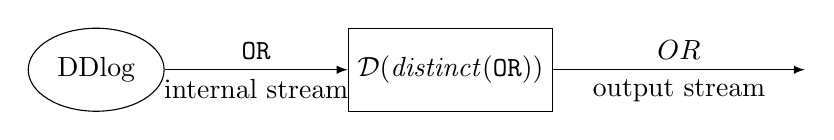
\begin{tikzpicture}[auto, node distance=4.5cm,>=latex]
    \node [block, shape=ellipse] (ddlog) {DDlog};
    \node [block, right of=ddlog] (block) {$\D(\distinct(\code{OR}))$};
    \node [output, right of=block] (output) {};
    \draw [draw,->] (ddlog) -- node {\code{OR}} (block) node [below,pos=0.5] {internal stream};
    \draw [->] (block) -- node {$OR$}(output) node [below,pos=0.5] {output stream};
\end{tikzpicture}

A DDlog declaration of \code{output relation OR[D]} declares a stream
$OR \in \stream{\Z[\code{D}]}$.  The elements of the stream are $OR$ are defined
by $OR = \D(\distinct(\code{OR}))$.

\subsection{DDlog operators}

All DDlog operators: join, group-by, aggregate, projection, etc., are
just particular instances of functions over multisets.  When computing
over streams DDlog just applies these functions to the streams
pointwise.  In this section we describe the semantics of these
operators over a multi-set; the semantics over streams is just lifted
pointwise.

\subsection{DDlog syntax}

A Datalog rule is a term of the form:

\begin{eqnarray*}
  rule &::=& atom \code{ :- } \mathit{RHSClauses}. \\
  atom &::=& C[X] \mbox{ where $C$ is a collection and $X$ is a tuple
    of names} \\
  \mathit{RHSClauses} &::=& \mathit{RHSClause} \\
  &|& \mathit{RHSClause}, \mathit{RHSClauses} \\
  \mathit{RHSClause} &::=& \code{not } atom \\
  &|& expr   \\
  &|& \code{var } name = expr \\
  &|& \code{var } name = \code{FlatMap}( expr ) \\
  &|& \code{var } name = expr \code{.groupby}( expr ) \\
\end{eqnarray*}

\subsection{Typing rules}

\code{X}: $T$

\subsubsection{Multiset semantics}

We use $\llbracket t \rrbracket$ to denote the semantics of a term
$t$.  The semantics of a $\mathit{RHSClauses}$ term is a mapping of
all live variables to a multisets of tuples values.  In a typing
environment $\Gamma = x_1 : T_1, x_2 : T_2, \ldots, x_m : T_m$, the
semantics of a \code{RHSClauses}

\end{document}
